\documentclass[11pt,openany]{article}

\input{algebra-note-preamble}
\input{tcolorbox}
\input{theorem}
\input{algebra-note-commands}
\usepackage{tikz}
\usepackage{tikz-3dplot}
\usepackage{amsmath}

\setstretch{1.25}
\begin{document}
\pagenumbering{arabic}
\begin{center}
	\huge\textbf{Projective Space}\\
	\vspace{0.5em}
	\large{Ji, Yong-hyeon}\\
	\vspace{0.5em}
	\normalsize{\today}\\
\end{center}
%\begin{figure}[h!]
%	\centering
%	\begin{tikzpicture}
%		% Draw sphere
%		\shade[ball color = gray!40, opacity = 0.4] (0,0) circle (2cm);
%		\draw (0,0) circle (2cm);
%		\draw (-2,0) arc (180:360:2 and 0.6);
%		\draw[dashed] (2,0) arc (0:180:2 and 0.6);
%		
%		% Lines meeting at a point (north pole)
%		\draw[thick] (-1.5, 1) -- (1.5, -1);
%		\draw[thick] (-1.5, -1) -- (1.5, 1);
%		\draw[thick, dashed] (0, 2) -- (0, -2);
%		
%		% Point at infinity (north pole)
%		\filldraw[fill=black] (0,2) circle (2pt);
%		
%		% Labels
%		\node at (0,2.3) {North Pole (Point at Infinity)};
%		\node at (2.5,1) {$l_1$};
%		\node at (2.5,-1) {$l_2$};
%		\node at (-0.5,0) {$l_3$};
%	\end{tikzpicture}
%	\caption{Projective Plane Representation with Lines Meeting at Infinity}
%\end{figure}

\begin{figure}[h!]
	\centering
	\begin{tikzpicture}[scale=1.5]
		% Draw the axes
		\draw[thick,->] (0,0,0) -- (4,0,0) node[anchor=north east]{$x$};
		\draw[thick,->] (0,0,0) -- (0,5,0) node[anchor=north west]{$y$};
%		\draw[thick,->] (0,0,0) -- (0,0,3) node[anchor=south]{$x$};
		
		% Draw vectors
		\draw[thick, -stealth, blue] (0,0,0) -- (2,4,2) node[anchor=west]{$2\mathbf{v}$};
		\draw[thick, -stealth, red] (0,0,0) -- (1,2,1) node[anchor=west]{$\mathbf{v}$};
		\draw[thick, -stealth, green!75!black] (0,0,0) -- (0.5,1,0.5) node[anchor=west]{$0.5\mathbf{v}$};
		
		% Labels
		\node at (1,2,1) [circle,fill,inner sep=1.5pt]{};
		\node at (2,4,2) [circle,fill,inner sep=1.5pt]{};
		\node at (0.5,1,.5) [circle,fill,inner sep=1.5pt]{};
	\end{tikzpicture}
	\caption{In $\mathbb{R}^2$ (or $\mathbb{C}^1$), vectors \( \mathbf{v} \), \( 2\mathbf{v} \), and \( 0.5\mathbf{v} \) lie on the same line.}
\end{figure}
%\begin{tikzpicture}
%	% Draw the complex plane
%	\fill[gray!20] (-2,-2) rectangle (2,2);
%	\draw[thick,->] (-2,0) -- (2,0) node[anchor=north west] {Re};
%	\draw[thick,->] (0,-2) -- (0,2) node[anchor=south east] {Im};
%	
%	% Draw the sphere
%	\draw[thick] (5,0) circle (2cm);
%	\fill[gray!10] (5,0) circle (2cm);
%	
%	% North pole point
%	\fill[black] (5,2) circle (2pt) node[anchor=south] {Point at Infinity};
%	
%	% Equator and meridians
%	\draw[dashed] (3,0) arc[start angle=180, end angle=0, x radius=2cm, y radius=0.5cm];
%	\draw (3,0) arc[start angle=-180, end angle=0, x radius=2cm, y radius=0.5cm];
%	
%	\draw[dashed] (5,-2) -- (5,2);
%	\draw[dashed] (5,0) -- (7,0);
%	
%	% Label for the plane
%	\node at (0,-2.3) {Complex Plane $\mathbb{C}$};
%	
%	% Label for the sphere
%	\node at (5,-2.3) {Riemann Sphere $\mathbb{P}^1(\mathbb{C})$};
%	
%	% Line indicating stereographic projection
%	\draw[thick,->] (2.5,0.5) -- (4,0.5);
%%	\node at (3.3,0.8) {Stereographic Projection};
%\end{tikzpicture}
\vfill
\begin{center}
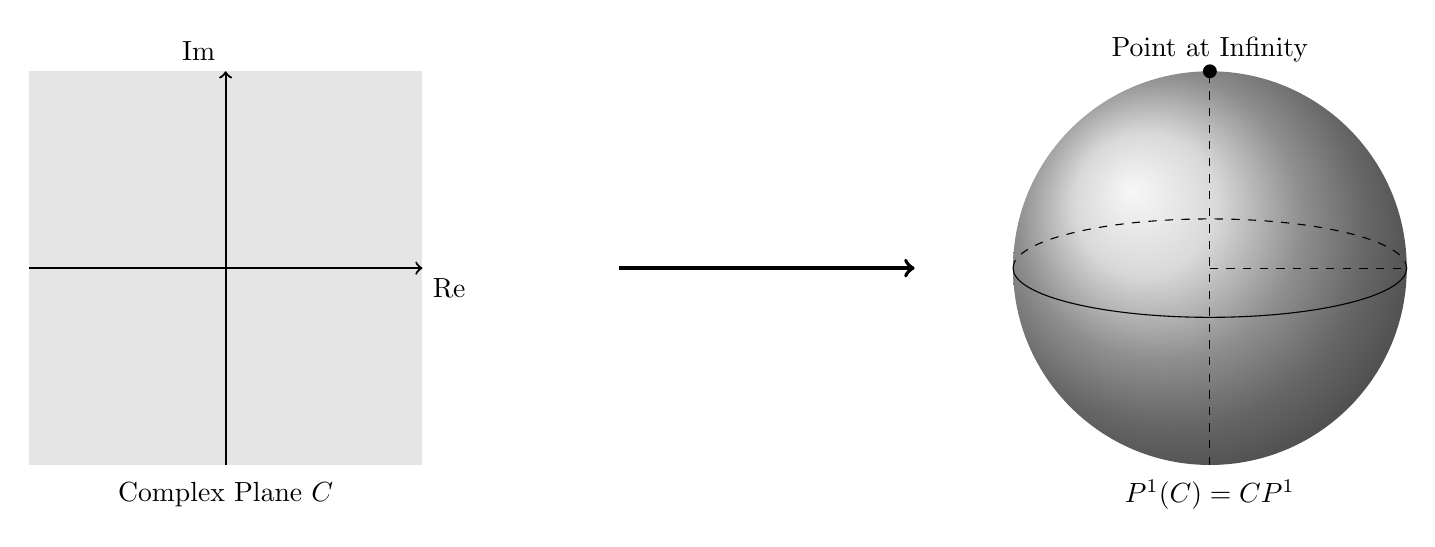
\begin{tikzpicture}[scale=1.25]
	% Draw the complex plane
	\fill[gray!20] (-2,-2) rectangle (2,2);
	\draw[thick,->] (-2,0) -- (2,0) node[anchor=north west] {Re};
	\draw[thick,->] (0,-2) -- (0,2) node[anchor=south east] {Im};
	
	% Draw the sphere with shading
	\shade[ball color=gray!40] (10,0) circle (2cm);
	
	% North pole point
	\fill[black] (10,2) circle (2pt) node[anchor=south] {Point at Infinity};
	
	% Equator and meridians
	\draw[dashed] (8,0) arc[start angle=180, end angle=0, x radius=2cm, y radius=0.5cm];
	\draw (8,0) arc[start angle=-180, end angle=0, x radius=2cm, y radius=0.5cm];
	
	\draw[dashed] (10,-2) -- (10,2);
	\draw[dashed] (10,0) -- (12,0);
	
	% Label for the plane
	\node at (0,-2.3) {Complex Plane $\mathbb{C}$};
	
	% Label for the sphere
	\node at (10,-2.3) {$\mathbb{P}^1(\mathbb{C})=\mathbb{C}\mathbb{P}^1$}; %Riemann Sphere 
	
	% Line indicating stereographic projection
	\draw[thick, line width=.5mm, ->] (4,0) -- (7,0);
%	\node at (3.3,0.8) {Stereographic Projection};
\end{tikzpicture}
\end{center}

\begin{center}
%\tdplotsetmaincoords{70}{120} % Set the viewing angle for the 3D plot
%\tdplotsetmaincoords{70}{30} % Set viewing angle
%\begin{tikzpicture}[tdplot_main_coords]
%	
%	% Sphere
%	\shade[ball color=gray!30, opacity=0.6] (0,0,2) circle (2);
%	\draw[dashed] (8,0) arc[start angle=180, end angle=0, x radius=2cm, y radius=0.5cm];
%	\draw (8,0) arc[start angle=-180, end angle=0, x radius=2cm, y radius=0.5cm];
%	
%	% Define points
%	\coordinate (N) at (0,0,4);   % North pole
%	\coordinate (S) at (0,0,0);   % South pole
%	\coordinate (A) at (2,0,0);   % Point on the equator
%	\coordinate (B) at (1,1.732,0); % Another point on the equator
%	\coordinate (C) at (0,2,0); % Another point on the equator
%	
%	% Draw the sphere's equator
%	\draw[dashed] (0,0,0) circle (2);
%	
%	% Lines for projection
%	\draw[thick] (N) -- (A);
%	\draw[thick] (N) -- (B);
%	\draw[thick] (N) -- (C);
%	
%	% Equatorial plane and lines
%	\draw[thick] (0,-2,0) -- (0,2,0);
%	\draw[thick] (-2,0,0) -- (2,0,0);
%	\draw[thick] (-1.5,-1.5,0) -- (1.5,1.5,0);
%	
%	% Projection Lines
%	\draw[dashed] (N) -- (S);
%	
%	% Stereographic projection lines (dashed for clarity)
%	\draw[dashed] (N) -- (A);
%	\draw[dashed] (N) -- (B);
%	\draw[dashed] (N) -- (C);
%	
%	% Sphere Axes
%	\draw[->] (0,0,0) -- (0,0,5) node[anchor=south]{$z$};
%	\draw[->] (-3,0,0) -- (3,0,0) node[anchor=west]{$x$};
%	\draw[->] (0,-3,0) -- (0,3,0) node[anchor=south]{$y$};
%	
%	% Labels
%	\node[above] at (N) {N};
%	\node[below] at (S) {S};
%	\node[right] at (A) {A};
%	\node[right] at (B) {B};
%	\node[right] at (C) {C};
%	
%\end{tikzpicture}
\end{center}
%\begin{figure}[h!]
%	\centering
%	\begin{tikzpicture}[scale=1.5]
%		% Define the radius of the sphere
%		\def\r{2}
%		
%		% Draw the sphere with semi-transparency
%		\shade[ball color = blue!10, opacity=0.5] (0,0) circle (\r);
%		
%		% Draw the equator
%		\draw (0,0) circle (\r);
%		\draw[dashed] (-\r,0) arc (180:360:\r cm and 0.6cm);
%		\draw (\r,0) arc (0:180:\r cm and 0.6cm);
%		
%		% Draw a plane that intersects the sphere
%		\begin{scope}
%			\clip (0,0) circle (\r); % Clipping for neat intersection
%			\fill[blue, opacity=0.5] (-2.5,-1) rectangle (2.5,3);
%		\end{scope}
%		
%		% Draw intersection line (great circle)
%		\draw[thick] (-2.5,1) -- (2.5,-1);
%		
%		% Add labels
%		\node at (0,\r+0.5) {North Pole};
%		\node at (0,-\r-0.5) {South Pole};
%		\node[fill=white] at (0,1) {Intersection Line};
%		\node at (2.2,-0.8) {Plane};
%		
%		% Points of intersection
%		\filldraw[fill=red] (-1.118,0.447) circle (2pt);
%		\filldraw[fill=red] (1.118,-0.447) circle (2pt);
%		\node at (-1.4,0.7) {Point A};
%		\node at (1.4,-0.7) {Point B};
%		
%	\end{tikzpicture}
%	\caption{Projective Plane \( \mathbb{P}^2 \) represented by a sphere, showing a plane intersecting as a great circle. Antipodal points (A and B) are identified.}
%\end{figure}
%\newpage
\defbox[Projective Space]{\begin{definition*}
Let \( \mathbb{K} \) be a field and $n\geq 0$. The \textbf{$\mathbf{n}$-dimensional projective space} over \( \mathbb{K} \), denoted \( \mathbb{P}(\mathbb{K}^{n+1}) \), is defined as the quotient:
\[
\mathbb{P}(\mathbb{K}^{n+1}) := (\mathbb{K}^{n+1} \setminus \{\textbf{0}\}) / \sim,
\]
where $\sim$ is an equivalence relation defined on $\mathbb{K}^{n+1}\setminus\set{\textbf{0}}$ by \[
\mathbf{v} \sim \mathbf{w} \iff \exists\lambda\in \mathbb{K} \setminus \{0\}\ \text{such that}\ \mathbf{v} = \lambda \mathbf{w}
\] for $\textbf{v},\textbf{w}\in\mathbb{K}^{n+1}$.
\end{definition*}}
\begin{remark*}
	$\mathbb{P}(\mathbb{K}^{n+1})$ is the set of lines through the origin in $\mathbb{K}^{n+1}$. These lines represent equivalence classes of non-zero vectors in $\mathbb{K}^{n+1}$, where two vectors are equivalent if they are scalar multiples of each other.
\end{remark*}
\begin{note}[Notation]
The projective space $\mathbb{P}(\mathbb{K}^{n+1})$ has dimension $n$. \begin{itemize}
	\item $\mathbb{P}(\mathbb{K}^{n+1}) = \mathbb{P}^n(\mathbb{K})$
	\item $\mathbb{P}(\mathbb{K}^{n+1}) = \mathbb{K}\mathbb{P}^n$
\end{itemize}
\end{note}
%\begin{tikzpicture}
%	
%	% Draw the sphere
%	\shade[ball color = gray!20, opacity = 0.4] (0,0) circle (3cm);
%	
%	% Draw the equator
%	\draw[dashed] (3,0) arc (0:180:3cm and 0.8cm);
%	
%	\draw (3,0) arc (0:-180:3cm and 0.8cm);
%	
%	% Draw meridians
%	\draw[dashed] (0,3) arc (90:270:0.8cm and 3cm);
%	\draw (0,3) arc (90:-90:0.8cm and 3cm);
%	
%	% Draw axes
%	\draw[->, thick] (-3.5,0) -- (3.5,0) node[anchor=west] {$\operatorname{Re}$};
%	\draw[->, thick] (0,-3.5) -- (0,3.5) node[anchor=south] {$\operatorname{Im}$};
%	
%	% North and South Poles
%	\filldraw[black] (0,3) circle (2pt) node[anchor=north] {North Pole ($\infty$)};
%	\filldraw[black] (0,-3) circle (2pt) node[anchor=south] {South Pole ($0$)};
%	
%	% Point on the equator
%	\filldraw[black] (3,0) circle (2pt) node[anchor=west] {$1$};
%	
%	% Labels
%%	\node at (0,0) {Equator};
%\end{tikzpicture}
%
%\begin{tikzpicture}
%	
%	% Draw the circle
%	\draw[thick] (0,0) circle (3cm);
%	
%	% Axes
%	\draw[->, thick] (-4,0) -- (4,0) node[anchor=west] {$x$};
%	\draw[->, thick] (0,-3.5) -- (0,3.5) node[anchor=south] {$y$};
%	
%	% Line through the origin (representative line)
%	\draw[thick, blue] (-3,-1.5) -- (3,1.5);
%	\node[blue] at (3,1.5) [anchor=west] {$(x,y)$};
%	
%	% Mark some points on the circle
%	\filldraw[black] (3,0) circle (2pt) node[anchor=north] {$[1,0]$};
%	\filldraw[black] (-3,0) circle (2pt) node[anchor=north] {$[-1,0]$};
%	\filldraw[black] (0,3) circle (2pt) node[anchor=east] {$[0,1]$};
%	\filldraw[black] (0,-3) circle (2pt) node[anchor=east] {$[0,-1]$};
%	
%	% Labels
%	\node at (0,-4) {$\mathbb{P}^1(\mathbb{R})$: Lines through the origin};
%	
%\end{tikzpicture}
%\begin{tikzpicture}
%	
%	% Draw the circle
%	\shade[ball color = gray!20, opacity = 0.4] (0,0) circle (3cm);
%	
%	% Draw the equator (horizontal line on the plane)
%	\draw[dashed] (-3,0) -- (3,0);
%	
%	% Draw the real line extended
%	\draw[->, thick] (-4,0) -- (4,0) node[anchor=west] {$\mathbb{R}$};
%	
%	% Mark the "infinity" point on the circle
%	\filldraw[black] (0,3) circle (2pt) node[anchor=south] {$\infty$};
%	
%	% Projection lines
%	\draw[dashed] (0,3) -- (2,0);
%	\draw[dashed] (0,3) -- (-2,0);
%	
%	% Two points on the real line and their projections
%	\filldraw[black] (2,0) circle (2pt) node[anchor=north] {$1$};
%	\filldraw[black] (-2,0) circle (2pt) node[anchor=north] {$-1$};
%	
%\end{tikzpicture}
%\begin{center}
%\begin{tikzpicture}
%	
%	% Draw axes
%	\draw[->, thick] (-4,0) -- (4,0) node[anchor=west] {$x$};
%	\draw[->, thick] (0,-4) -- (0,4) node[anchor=south] {$y$};
%	
%	% Lines through the origin
%	\draw[thick, line width = .75mm, blue] (-3,-3) -- (3,3);
%	\draw[thick, line width = .75mm, red] (-3,1.5) -- (3,-1.5);
%	\draw[thick, line width = .75mm, green!75!black] (-2.5,0) -- (2.5,0);
%	\draw[thick, line width = .75mm, orange] (0,-2.5) -- (0,2.5);
%	
%	% Labels
%	\node at (0,-4.5) {$\mathbb{P}(\R^2)=\mathbb{P}^1(\mathbb{R})=\R\mathbb{P}^1$};
%	
%\end{tikzpicture}
%\end{center}

%\begin{figure}[h!]
%	\centering
%	\begin{tikzpicture}[scale=2.5]
%		% Define the radius of the sphere
%		\def\r{1}
%		
%		% Draw the sphere
%		\shade[ball color=blue!10!white,opacity=0.6] (0,0) circle (\r);
%		\draw (0,0) circle (\r);
%		\draw[dashed] (0,-\r) arc (270:450:\r cm and 0.3cm);
%		\draw[dashed] (0,-.3) arc (90:270:\r cm and 0.3cm);
%		
%		% Stereographic projection lines
%		\draw[dotted] (0, \r) -- (-\r, -\r/2);
%		\draw[dotted] (0, \r) -- (\r, -\r/2);
%		
%		% Points on the sphere
%		\filldraw[fill=red] (0, \r) circle (1pt) node[above] {Infinity};
%		\filldraw[fill=red] (\r/2, -\r/2) circle (1pt) node[below] {z};
%		\filldraw[fill=red] (-\r/2, -\r/2) circle (1pt) node[below] {w};
%		
%		% Add labels
%%		\node at (1.2*\r, 0) {Equator (Real axis)};
%%		\node[fill=white, inner sep=1pt] at (0,-1.2*\r) {Southern Hemisphere (Imaginary axis)};
%		
%	\end{tikzpicture}
%	\caption{Visualization of \( \mathbb{P}^1(\mathbb{C}) \) using the Riemann Sphere. Points z and w on the complex plane are mapped onto the sphere, with the north pole representing the point at infinity.}
%\end{figure}

\iffalse
\section*{Definition of Projective Space}

Projective space \( \mathbb{P}^n \) over a field \( \mathbb{K} \) is defined as the set of lines through the origin in \( \mathbb{K}^{n+1} \). These lines represent equivalence classes of non-zero vectors in \( \mathbb{K}^{n+1} \), where two vectors are considered equivalent if they are scalar multiples of each other. The formal definition is given by:
\[
\mathbb{P}^n(\mathbb{K}) = ( \mathbb{K}^{n+1} \setminus \{0\} ) / \sim
\]
where \( \sim \) is the equivalence relation defined by \( \mathbf{v} \sim \mathbf{w} \) if there exists a non-zero scalar \( \lambda \in \mathbb{K} \) such that \( \mathbf{v} = \lambda \mathbf{w} \).

\section*{Homogeneous Coordinates}

A point in \( \mathbb{P}^n \) is represented by a tuple of \( n+1 \) coordinates, not all zero, modulo the equivalence relation of proportionality:
\[
[x_0: x_1: \cdots : x_n]
\]
These coordinates are not unique; multiplying all coordinates by a non-zero scalar \( \lambda \) yields the same point in projective space:
\[
[x_0: x_1: \cdots : x_n] = [\lambda x_0: \lambda x_1: \cdots : \lambda x_n]
\]

\section*{Properties of Projective Space}

\begin{itemize}
	\item \textbf{Extension of Euclidean Space:} Projective space extends Euclidean space \( \mathbb{R}^n \) by adding "points at infinity" for each direction, simplifying many geometric proofs and concepts.
	\item \textbf{Invariance under Projection:} Projective transformations preserve lines and collinearity, represented by invertible matrices modulo scalar multiples.
	\item \textbf{Topology:} Projective space can be endowed with a topology, typically the quotient topology from \( \mathbb{K}^{n+1} \). Over the real or complex numbers, projective spaces are compact.
	\item \textbf{Projective Varieties:} A projective variety is defined as the zero set of a collection of homogeneous polynomials, providing a natural setting for studying polynomial equations in algebraic geometry.
\end{itemize}

\section*{Projective Geometry}

Projective geometry studies properties of figures invariant under projective transformations, featuring classical results such as Desargues' Theorem and Pappus's Theorem, and interpreting concepts like duality within its framework.

\section*{Example: Projective Plane}

The projective plane \( \mathbb{P}^2 \) consists of lines through the origin in three-dimensional space \( \mathbb{K}^3 \), visualized as a sphere where each point and its antipodal point are identified.

\section*{Core Definitions and Properties}

\begin{definition}[Projective Space]
	Let \( \mathbb{K} \) be a field. The \textit{n-dimensional projective space} over \( \mathbb{K} \), denoted \( \mathbb{P}^n(\mathbb{K}) \), is the set of lines through the origin in \( \mathbb{K}^{n+1} \). Formally, it is defined as the quotient:
	\[
	\mathbb{P}^n(\mathbb{K}) = (\mathbb{K}^{n+1} \setminus \{0\}) / \sim
	\]
	where \( \mathbf{v} \sim \mathbf{w} \) if \( \mathbf{v} = \lambda \mathbf{w} \) for some \( \lambda \in \mathbb{K} \setminus \{0\} \).
\end{definition}

\begin{definition}[Homogeneous Coordinates]
	A point in \( \mathbb{P}^n(\mathbb{K}) \) is represented by \textit{homogeneous coordinates}:
	\[
	[x_0 : x_1 : \dots : x_n]
	\]
	where \( (x_0, x_1, \dots, x_n) \in \mathbb{K}^{n+1} \setminus \{0\} \), and:
	\[
	[x_0 : x_1 : \dots : x_n] = [\lambda x_0 : \lambda x_1 : \dots : \lambda x_n] \quad \text{for all } \lambda \in \mathbb{K} \setminus \{0\}.
	\]
\end{definition}

%\begin{property}[Compactness and Continuity]
	The projective space \( \mathbb{P}^n(\mathbb{K}) \) is compact when \( \mathbb{K} = \mathbb{R} \) or \( \mathbb{C} \). Moreover, it carries a natural topology induced by the quotient of the standard topology on \( \mathbb{K}^{n+1} \).
%\end{property}

\begin{theorem}[Invariance under Projective Transformations]
	Let \( f: \mathbb{P}^n \rightarrow \mathbb{P}^n \) be a projective transformation represented by an invertible matrix \( A \in \text{GL}_{n+1}(\mathbb{K}) \). Then \( f \) preserves lines and collinearity, and is defined up to a scalar multiple.
\end{theorem}

\section*{Example: Projective Plane}

\begin{example}
	The projective plane \( \mathbb{P}^2(\mathbb{K}) \) is defined by:
	\[
	\mathbb{P}^2(\mathbb{K}) = (\mathbb{K}^3 \setminus \{0\}) / \sim
	\]
	where points \([x:y:z]\) represent lines through the origin in \( \mathbb{K}^3 \). This plane includes the entire affine plane \( \mathbb{K}^2 \) plus a line at infinity for each class of parallel lines.
\end{example}
\fi

\end{document}
